\graphicspath{{chapters/07/}}
\chapter{Molecular physics}
\section{The Born-Oppenheimer Approximation}
Molecular physics expalins the origin of chemical bonds and makes it possible to understand quantum chemistry calculations. Chemistry can be represented by an "unsolvable" Schr\"odinger equation:\\
\[
\bigg[-\sum_{q=1}^{N_{\alpha}}\frac{\hbar^2}{2m_{\alpha}}\cdot\nabla_{\alpha}^2
-\sum_{i=0}^{N_e}\frac{\hbar^2}{2m_e}\cdot\nabla^2_i
+V[\{\vec{R}\}_{\alpha},\{\vec{r_i}\}_i]\bigg]=E\Psi[\{\vec{R}\}_{\alpha},\{\vec{r}\}_i]
\]
\[
V[\{\vec{R}\}_{\alpha},\{\vec{r}_i\}]=\bigg(\sum_{i<j}\frac{e^2}{|\vec{r_i}-\vec{r_j}|}
+\sum_{\alpha<\beta}\frac{z_{\alpha}z_{\beta}e^2}{|\vec{R_{\alpha}}-\vec{R_{\beta}}|}
-\sum_{i,\alpha}\frac{e^2z_{\alpha}}{|\vec{r_i}-\vec{R_{\alpha}}|}\bigg)\]
In order, the different parts of the equation represent:
\begin{enumerate}
	\item $-\sum_{q=1}^{N_{\alpha}}\frac{\hbar^2}{2m_{\alpha}}\cdot\nabla_{\alpha}^2$,  Kinetics of nuclei
	\item $-\sum_{i=0}^{N_e}\frac{\hbar^2}{2m_e}\cdot\nabla^2_i$,  Kinetics of electrons
	\item $\sum_{i<j}\frac{e^2}{|\vec{r_i}-\vec{r_j}|}$,  Repulsive coulombic interaction between electrons
	\item $\sum_{\alpha<\beta}\frac{z_{\alpha}z_{\beta}e^2}{|\vec{R_{\alpha}}-\vec{R_{\beta}}|}$,  Repulsive coulombic interaction between nuclei
	\item $-\sum_{i,\alpha}\frac{e^2z_{\alpha}}{|\vec{r_i}-\vec{R_{\alpha}}|}$,  Attractive coulombic interaction between nucleus and electrons
	\item Curly brackets represent the collection of all r and R
\end{enumerate}
This equation can be approximated by considering that protons are much bigger and slower than electrons, and therefore are fixed. The Born-Oppenheimer approximation divides these operations in two (\textbf{decoupling}).\\
\newline
We can implement a \textit{divide et impera} approach:\\
\textbf{1)} Study the electronic problem at fixed nuclear configuration (i.e. ignoring the kinetic energy of the nuclei).\\
The first fragment is ignored (no motion, no kinetic energy) and the coulombic repulsion becomes constant consequently. Nuclei bind only when they are close to each other.
\[
\bigg[-\sum_{i=0}^{N_e}\frac{\hbar^2}{2m_e}\cdot\nabla^2_i
+\sum_{i<j}\frac{e^2}{|\vec{r_i}-\vec{r_j}|}
-\sum_{i,\alpha}\frac{e^2z_{\alpha}}{|\vec{r_i}-\vec{R_{\alpha}}|}\bigg]\cdot\Psi[\{\vec{R}\}_{\alpha},\{\vec{r}\}_i] =E[\{R_{\alpha}\}]\Psi[\{\vec{R}\}_{\alpha},\{\vec{r}\}_i]
\]
Where $E[\{R_{\alpha}\}]$ is the energy of the system at a fixed nuclear position, ${R_{\alpha}}$ represents the contributions of the electrons to the potential energy.\\
The energy eigenvalue describes the electron density around the nuclei at fixed nuclei positions. The fact that there are electrons moving increases the overall potential energy (repulsive interactions), electrons can lower their higher potential energy by tunneling to another nucleus with Pauli symmetry. This lowers the total energy of the system and creates bonds.\\ 
Note that this is not a "charge-driven" attraction, but a phenomenon driven by quantum tunneling and Pauli's symmetry. 
\newline
\textbf{2)} Solve the dynamics of the nuclei based on their own coulombic interactions and electrons effect.
\[
\bigg[-\sum_{q=1}^{N_{\alpha}}\frac{\hbar^2}{2m_{\alpha}}\cdot\nabla_{\alpha}^2
+\sum_{\alpha<\beta}\frac{z_{\alpha}z_{\beta}e^2}{|\vec{R_{\alpha}}-\vec{R_{\beta}}|}+E|\{R_\alpha\}| \bigg]\varphi(|R|)=\varepsilon\varPhi(\{R\})
\]
Note that $\varepsilon$ is a value, not a function, it does not depend on any parameter.\\
The quantum effect becomes weaker as the weight of the system increases. To describe a many-body system, I can replace this Schr\"odinger equation with a Newtonian equation.\\
\[
M_\alpha\frac{d^2}{dt^2}R_\alpha(t)=-\nabla_\alpha(E(R)+E_t(R))
\]
This equation is fine for describing \textbf{classical molecular simulations}. We loose the quantum effects of the nuclei (protonation - quantum tunneling of protons, chemical reactions...), and often for molecules a classical formulation is enough.

\section{The H$_2$ molecule}
We are given two protons (a,b) and two electrons (1,2). Consider the structure of the electronic wave function as $\Psi(\vec{r_1},\vec{r_2},s_1^z,s_2^z,(\vec{R_a},\vec{R_b}))$ where $(\vec{R_a},\vec{R_b})$ is a fixed external parameter because of the Born-Oppenheimer approximation (distance between nuclei). A schematic draw of the problem is depicted in figure \ref{fig:h2}.\\
\begin{figure}[htbp!]
	\centering
	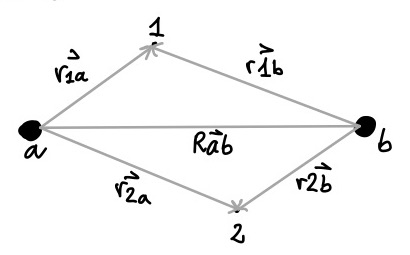
\includegraphics[scale=0.30]{img_8}
	\caption{A representation of the $H_2$ molecule, given the Born-Oppenheimer approximation.}
	\label{fig:h2}
\end{figure}
\newline
The system can be firstly represented as two atoms at a large distance that approach slowly to each other, generating a linear combination of mean wave functions. The electrons are in a superposition of states when they start interacting, so the resulting H-H chemical bond is actually an entangled electron tunneling.
\[
\Psi(\vec{r_1},\vec{r_2},s_1^z,s_2^z,(\vec{R_a},\vec{R_b}))=\Psi_{\text{spatial}}(\vec{r_1},\vec{r_2})\otimes\Psi_{\text{spin}}(s_1^z,s_2^z)=\Phi\otimes\mathcal{X}
\]
The wave-function can be factorized, as the Hamiltonian is separable (i.e. does not depend on the spin).\\
Spins can be $\ket{\uparrow\uparrow}$, $\ket{\downarrow\downarrow}$, $\ket{\uparrow\downarrow}$, and $\ket{\downarrow\uparrow}$. Since electrons are fermions, the two spins' product must be antisymmetric, hence one of the two spins must be antisymmetric and the other one must be symmetric (the two possibilities are \textit{i}) spatial symmetry and spin antisymmetric, \textit{ii}) spatial antisymmetry and simmetric spin). Symmetry can be evaluated in entangled states, too. 

\begin{description}
   \item[Symmetric spin] ($J=1$): $\ket{\uparrow\uparrow}$, $\ket{\downarrow\downarrow}$, $\frac{\ket{\uparrow\downarrow}+\ket{\downarrow\uparrow}}{\sqrt{2}}$ also called \textbf{triplet state} (quantum state of a system with a spin quantum number $s=1$), molecule bends in Stern-Gerlach.\\
   \item[Antisymmetric spin] ($J=0$): $\frac{\ket{\uparrow\downarrow}-\ket{\downarrow\uparrow}}{\sqrt{2}}$ also called \textbf{singlet state} (total spin angular moment $s=0$), molecule doesn't bend in Stern-Gerlach.\\
\end{description}

The result is that a combination of two spin-1/2 particles can carry a total spin of 1 or 0, depending on whether they occupy a triplet or singlet state.\\

Now we can generate now a model through a variational ansatz:
\[
\Psi=\Phi \mathcal{X}=\begin{cases}
\Psi_1=\Phi_S \mathcal{X}_A = \frac{1}{\sqrt{2}} \big(\varphi_a(r_{1a}) \varphi_b (r_{1b})+\varphi_a (r_{2a}) \varphi_b (r_{2b})\big) \otimes\frac{\ket{\uparrow\downarrow}-\ket{\downarrow\uparrow}}{\sqrt{2}}\\
\Psi_2=\Phi_A\mathcal{X}_S = \frac{1}{\sqrt{2}} \big(\varphi_a(r_{1a}) \varphi_b (r_{1b})+\varphi_a (r_{2a}) \varphi_b (r_{2b})\big) \otimes\frac{\ket{\uparrow\downarrow}+\ket{\downarrow\uparrow}}{\sqrt{2}}\\
\end{cases}
\]
The latter is a mean field model where E1 lives in P1 and E2 lives in P2.\\
By the variational principle, the wavefunction with the lowest value of energy is the one that best approximates the H$_2$ atom.\\
\[
\hat{H}=-\frac{\hbar^2}{2m}\nabla_n^2-\frac{\hbar^2}{2m}\nabla_e^2-\frac{e^2}{|r_1a|}-\frac{e^2}{|r_1b|}-\frac{e^2}{|r_2a|}-\frac{e^2}{|r_2b|}-\frac{e^2}{|R_ab|}
\]
Even if spin is not involved in the Hamiltonian and eventually results in $\braket{\hat{S}}{\hat{S}}=1$, the sign of the expected value of the Hamiltonian depends on the spin symmetry, because spatial value and spin symmetry are entangled.
\[E_1=\langle{\Psi_1\,|\,\hat{H}\,|\,\Psi_1}\rangle =\langle{\Phi_S\,|\,\hat{H}\,|\,\Phi_S}\rangle\]
\[E_2=\langle{\Psi_2\,|\,\hat{H}\,|\,\Psi_2}\rangle=\langle{\Phi_A\,|\,\hat{H}\,|\,\Phi_A}\rangle\]
We must solve, then,
\[
E_1=\frac{1}{2}\int d\vec{r_1}\int d\vec{r_2}\,\big[\varphi(|\vec{r_1}-\vec{R_a}|)\varphi(|\vec{r_2}-\vec{R_b}|)+\varphi(|\vec{r_1}-\vec{R_b}|)\varphi(|\vec{r_2}-\vec{R_a}|)\big](\hat{H})(\Phi_S)
\]
and same for $E_2$. I have two 6-dimensions functions in 6-dimensions integrals.\\
Results are different whether I solve for the first or second electron.\\
%This is the result that is obtained when the two atoms are infinitely far.\\
%\[
%\braket{\,|\,\hat{H}\,|\,}_{S/A}=2E_0\pm\text{stuff}
%\]
%Else, if the two atoms start to approach,
%\[
%\braket{\,|\,\hat{H}\,|\,}_{S/A}=\frac{e^2}{R_{ab}}\pm\text{separated ground states}
%\]
We obtain two different functions, depicted in figure \ref{fig:variational}:
\begin{itemize}
	\item \textbf{Symmetric spatial function}: spin 0 state, has a lower energy value that corresponds to an optimal distance between the two nuclei $\bar{R}$. It allows different calculable energy levels, bond oscillations and strength. Important to notice is that \textbf{quantum symmetry} (state s=0) is key to the binding of atoms. 
	\item \textbf{Antisymmetric spatial function}: goes against the variational approximation, but technically is a right solution from a quantum mechanical point of view.
\end{itemize}
\begin{figure}[htbp!]
	\centering
	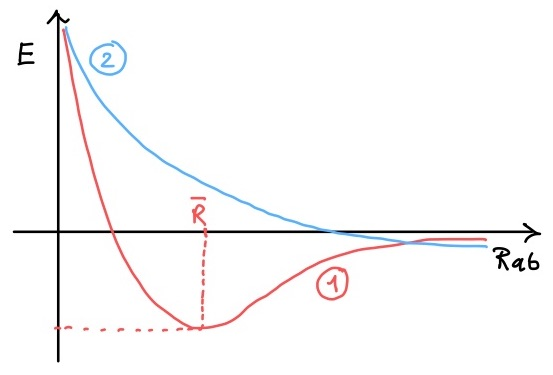
\includegraphics[scale=0.30]{img_9}
	\caption{The toal energy is: $|E \rangle = \langle \psi | H | \psi \rangle = 2E_0 + \frac{e^2}{R_{ab}} \text{+ other factors}$. $E_0$ corresponds tot the energy of two atoms infinitely far away from each others, while $\frac{e^2}{R_{ab}}$ acts when the two atoms start to approach.}
	\label{fig:variational}
\end{figure}
\section{Electronic structure calculation methods}
When choosing the best method to obtain an electronic structure, some evaluations have to be made regarding the accuracy of the calculation vs the computational cost of the operation. The first approximation to be chosen is always the most important and it determines the further steps that need to be taken. It is very important then to consider strategic decisions in computational sciences.\\
\begin{figure}[htbp!]
	\centering
	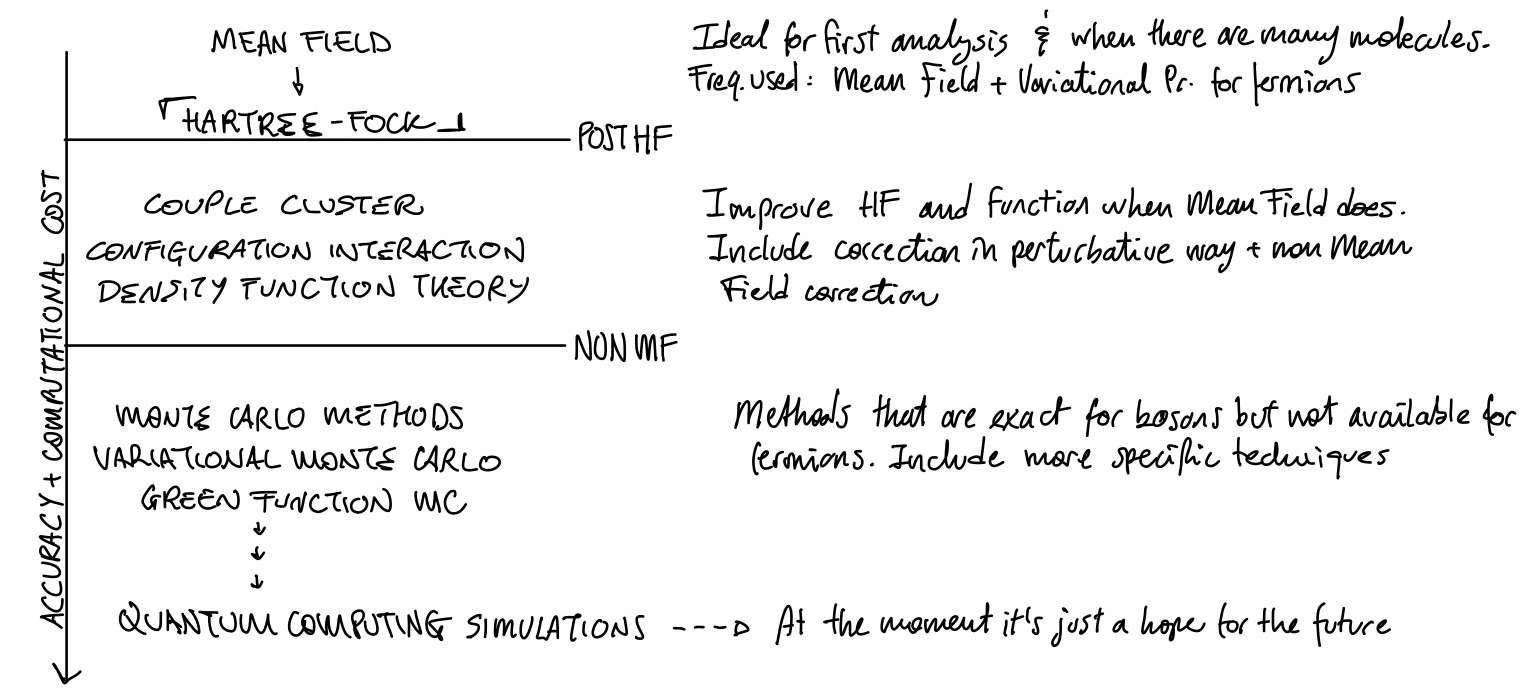
\includegraphics[scale=0.30]{img_13}
\end{figure}
\newline
I also have \textbf{EXACT DIAGONALIZATION (TRUNCATED BASIS)} that is very precise, but can't be used with system with more than 5 or 6 particles at the same time.\\
For biological system, chemical accuracy is important as long as the error is not dramatic (slightly change of temperature can dramatically change the system). A simulation is acceptable when $K_BT < 1.5\text{ KJ/mol} \div 2.4 \text{ KJ/mol}$.\\
For macromolecules in biology, very accurate DFT are performed. The problem is that it's very difficult to predict Van Der Waals forces, since they are polynomial and DFT uses exponentials.\\
The general goal is using classical equations to predict quantum-mechanics-descripted movements.\\
\subsubsection{Hartree-Fock Method}
Hartree-Fock method is a method of approximation for the determination of the wave function and the energy of a quantum many-body system in a stationary state that combines Mean Field Approximation, Fermi symmetry, and the Variational Principle.\\
The method uses the Slater matrix's determinant to approximate a set of $N$ fermions.
\[
\Psi(q_1...q_n)=\frac{1}{\sqrt{2}}
\begin{pmatrix}
\phi_1(r_1)&...&\phi_n(r_1)\\
... & &...\\
\phi_1(r_m)&...&\phi_n(r_m)
\end{pmatrix}
\]
I do not expect to find $\Psi(q_1...q_n)$, I can say it is the result of an equation and so calculate the energy by using the Variational Principle with $E=\braket{\Psi\,|\,E\,|\,\Psi}$ and minimize $E$ with respect to$\psi(q)$ (a single-particle function) under the costraint of normalization ($\braket{\psi\,|\,\psi}=1$)\\
Costraint minimization is operated with \textbf{Lagrange multipliers}: I consider a system of equations $f(x_1...x_n)$ where I can calculate the minimum and the maximum with the application of the gradient $\nabla f=0$.\\

We eventually obtain the \textbf{Hartree Equation}, representing \ul{one electron interacting with a probability cloud}. It is a symmetric system (valid for bosons, since they have classical limits and can be represented as shown without further additions):
\[
\bigg(-\frac{\hbar^2}{2m}\nabla^2_i-\frac{Z}{r_i}\bigg)\Phi_\lambda(\vec{r_i})+\sum_\mu \sum_{j \neq i} \int\,d^3\vec{r_j}\bigg(\Phi^*_\mu(\vec{r_j})\Phi_\mu(\vec{r_j})\frac{1}{|r_i-r_j|}\Phi_\lambda(\vec{r_i})\bigg)=E\Phi_\lambda(\vec{r_i})
\]
In particular:
\begin{itemize}
	\item $-\frac{Z}{r_i}$ is the coulombic attraction for a single nucleus (atomic physics version)
	\item $\Phi_\lambda(\vec{r_i})$ represents orbital position of the electron + spin. The number of electrons is the number of equations that need to be solved
	\item $\mu$ is the orbital index that changes the wave function
	\item $\Phi^*_\mu(r_j)\Phi_\mu(r_j) = \rho_\mu^{(i)}(r_j)$ is the electron density + density of charge around it (probability density) with sum of all electrons in all orbitals ($\mu$)
\end{itemize}
Fermi symmetry introduces Slater determinant that is also called \textbf{exchange term} (\textbf{Fock equation}). This introduction implies that I cannot bring two electrons with the same spin in the same orbital. The wave function collapses to zero and I have repulsion between the electrons.\\
\[
\text{HARTREE EQN.}+
\sum_\mu \sum_{j \neq i} \int\,d^3\vec{r_j}\bigg(\Phi^*_{\mathcolorbox{yellow}{\mu}}(\vec{r_j})\Phi_{\mathcolorbox{yellow}{\lambda}}(\vec{r_j})\frac{1}{|r_i-r_j|}\Phi_{\mathcolorbox{yellow}{\mu}}(\vec{r_i})\bigg)=E\Phi_\lambda(\vec{r_i})
\]
This implies that the electron density factor of Hartree equation is not present anymore, the two particles are in a different state. At the same time $\Phi_\mu(r_i)$ becomes Fock's generalization exchange term for fermions.\\

This equation though is non linear ($\Phi^3$), so many quantum mechanics properties can't be applied to HF.\\
The computational cost doesn't change over the introduction of the exchange term even if it has a three-dimensional integral.\\
I can't expand the equation on a different basis, I must use SELF CONSISTED METHODS/APPROACHES that are \ul{iterative procedures operated until the function converges.}
\begin{enumerate}
	\item (Guess) $\Phi_\lambda (\vec{r})$
	\item Compute $\rho_\mu^{(1)}(\vec{r})$ and $\rho_\mu^{(2)}(\vec{r})$ as they are numerical values
	\item Insert $\rho_\mu^{(1)}(\vec{r})$ and $\rho_\mu^{(2)}(\vec{r})$ into HF equation, resulting in a conventional linear Schr\"odinger equation.
	\item Solve HF equation and get a more accurate wave function $\Phi_\lambda (\vec{r})$
	\end{enumerate}
The obtained $\Phi_\lambda (\vec{r})$ is a better guess than the initial one so I use the latter obtained again for point 1 and recompute the density. I continue until I converge. Usually I have a single minimum. \\
I can use SELF CONSISTENT FIELDS to compute HF equation but they are computationally expensive, they can be used for parallel computing. \\

I can further use HF equation with SEMI EMPIRICAL METHODS with coefficients in front of direct and exchange terms that can weight the two terms in order to better match the experiment. I usually use HF to build the expansion of the eigenfunction or in quantum computing.\\

\subsection{Density Function Theory (DFT)}
Variational scheme that in principle can yield the exact result,  but in practice needs heuristic input/approximation. Over the made assumptions, I can have excellent results. I need simple inputs for the perfect compromise between accuracy and computational cost.\\
This theory is not based on the wave function computation, but on the \textbf{density function computation}.\\
\[
 \text{Density operator:}\hat{\rho}(\vec{r})=\sum_{i=1}^{N_0}\delta(\vec{r}-\vec{r_i})\]
 \[
\text{Expectation value, assuming} \braket{\Psi\,|\,\Psi}=1 \text{:}\, \braket{\Psi\,|\,\hat{\rho}(\vec{r})\,|\,\Psi}=\sum_i \int\,d\vec{r_1}...d\vec{r_{N_e}}\bigg(\Psi^*(\vec{r_1}-\vec{r_{N_e}})\delta(\vec{r}-\vec{r_i})\Psi(\vec{r_1}-\vec{r_{N_e}})\bigg)
\]
\[
\braket{\Psi\,|\,\hat{\rho}(\vec{r})\,|\,\Psi}=n(\vec{r})
\]
which is the probability of finding any electron at the point $r$. This concept is shown in the following picture,  where blue is low electron density and red is high electron density.\\
\begin{figure}[htbp!]
	\centering
	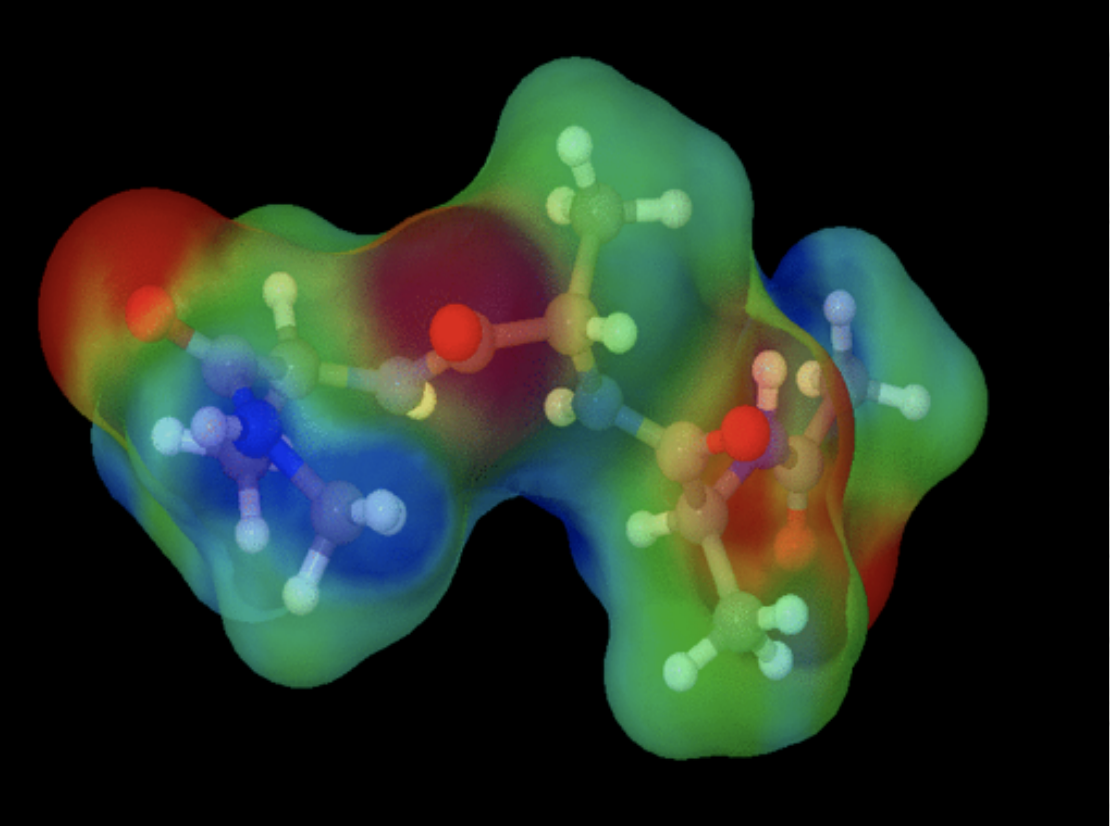
\includegraphics[scale=0.30]{img_14}
\end{figure}
\newline
\ul{OBS}: $n(\vec{r})$ is a so-called \textbf{SINGLE-BODY DENSITY}, it doesn't tell me the same information of the wave function (in fact $\hat{\rho}(\vec{r})$ reduces it when compared to $\Psi$). For any Hamiltonian there is one and only single-body density.\\

Hochenberg and Kohn have elaborated two theorems that show that the ground state and excited states' properties of a system (quantum manybody system)\marginpar{\textit{determined by some sort of *quantum magic*, cit.}} are entirely determined by a single-body wavefunction $n(\vec{r})$.\\
Mind that the quantum electronic structure calculation problem is:
\[
\hat{H}=-\frac{\hbar^2}{2m}\sum_i^{N_e}\nabla_i^2+\frac{1}{2}\sum_{i\neq j} \frac{e^2}{|r_i-r_j|}+\sum_i^{N_e}V_{ext}(\vec{r_i})
\]
Te last term is the interaction between single electrons and nuclei. IN BO approximation this was the external potential because nuclei were fixed.\\

\ul{THEOREM 1)} For any system of interacting particles, the external potential is determined uniquely by the ground state one-body density.
\[n_o(\vec{r})=\braket{\Psi\,|\,\hat{\rho}(\vec{r})\,|\,\Psi}\]

$\rightarrow\,\,$\ul{Corollary}: All wavefunctions (ground state, first excited state, all eigenstates of $\hat{H}$) are fully determined by $n_0(\vec{r})$\\

\ul{THEOREM 2)} A functional $E[n_0]$ can be defined such that the minimum of this functional with respect to $n_0(\vec{r})$ provides the exact $n_0(\vec{r})$ and $E_0$ (ground state energy).\\

\ul{OBS}: A function: $f: x \rightarrow f(x)$ ($x$ is a variable, $f(x)$ is a number)\\
A functional: $E[f]: f(x) \rightarrow E[f]$ ($f(x)$ is a function of operators, $E[f]$ is a number). Examples of functionals are definite integrals or expectation values of operators.\\
Anyway, from Ritz Theorem we know that the minimum of the functional of the wave function (i.e., the expectation value of the Hamiltonian) is the exact ground state.\\

I can define/is it possible to define a functional such as the minimum of the functional is the exact value of the ground state energy. Differently from Ritz Theorem, here the functional is not given and not referred to the wave function. One body density's functional's minimum is the exact ground state energy of the problem $\forall$ Hamiltonians.\\

These two are existent theorems, they do not provide any solution, usually they are complemented with ways to build the right functional to solve the problem.\\
\begin{figure}[htbp!]
	\centering
	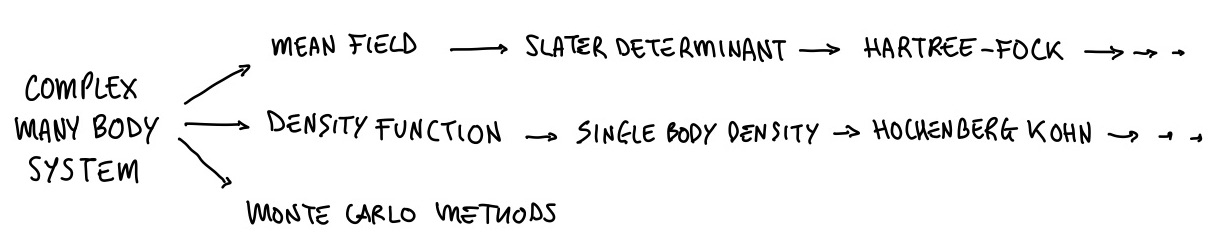
\includegraphics[scale=0.30]{img_15}
\end{figure}

\subsection{QM-MM Schemes}
QM-MM = Quantum Mechanics, Molecular Mechanics. These schemes are used for large molecular models and chemical reactions studies (e.g., enzymatic reactions).\\
QM is applied to the region of interest so to have the computational effort only where needed,  while classical molecular mechanics is applied elsewhere and an hybrid method is used at the threshold of the two regions.\\
The difficulty is presented when considering thermodynamics. The more degrees of freedom, the more entropy.\\
